\begin{frame}
\frametitle{\small $G_{I}$ from VCCI, stresses extracted on fiber surface, $\delta=3.0^{\circ}$}
\vspace{-0.75cm}
\centering
\captionsetup[figure]{font=scriptsize,labelfont=scriptsize}
\begin{figure}[!h]
\centering
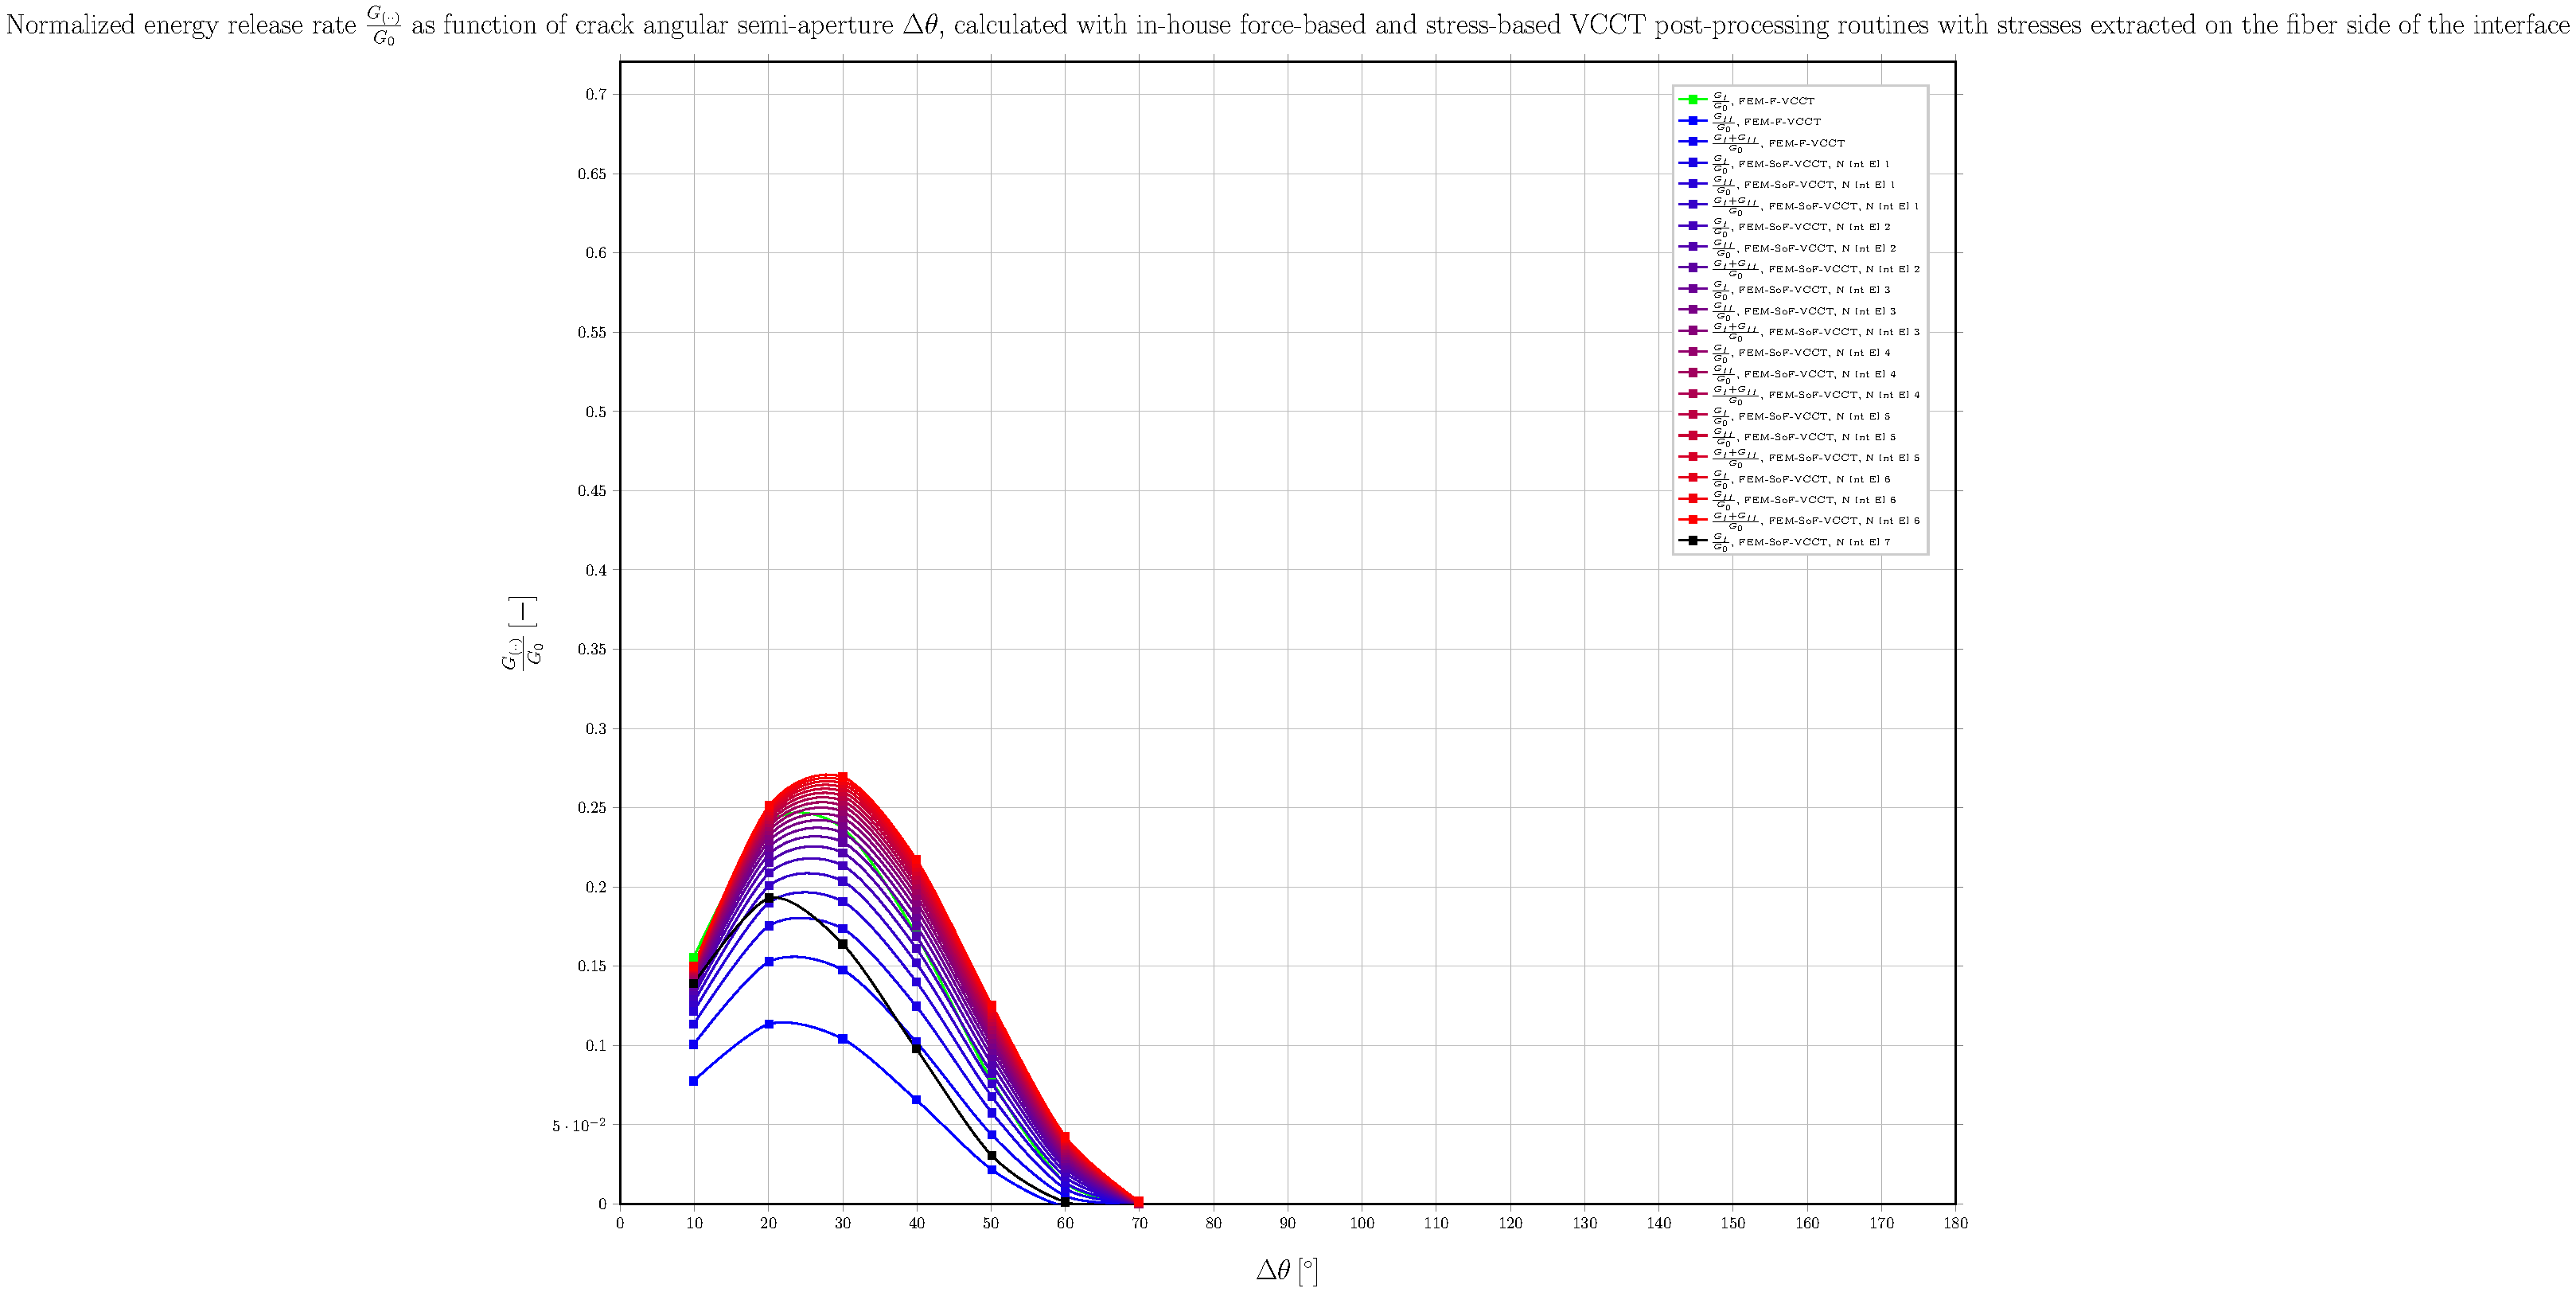
\includegraphics[height=0.7\textheight]{2017-07-25_AbqRunSummary_SmallStrain_D03/pdf/2017-07-25_AbqRunSummary_SmallStrain_D03_F-SoF-VCCT_GI.pdf}
  \caption{\scriptsize Fading from blue to red for increasing number of integration elements, Virtual Crack Closure Integral (VCCI) from FEM results; in green VCCT from FEM results; in black BEM results.}
  \label{fig:res1}
\end{figure}
\end{frame}
%%%%%%%%%%%%%%%%%%%%%%%%%%%%%%%%%%%%%
\begin{frame}
\frametitle{\small $G_{II}$ from VCCI, stresses extracted on fiber surface, $\delta=3.0^{\circ}$}
\vspace{-0.75cm}
\centering
\captionsetup[figure]{font=scriptsize,labelfont=scriptsize}
\begin{figure}[!h]
\centering
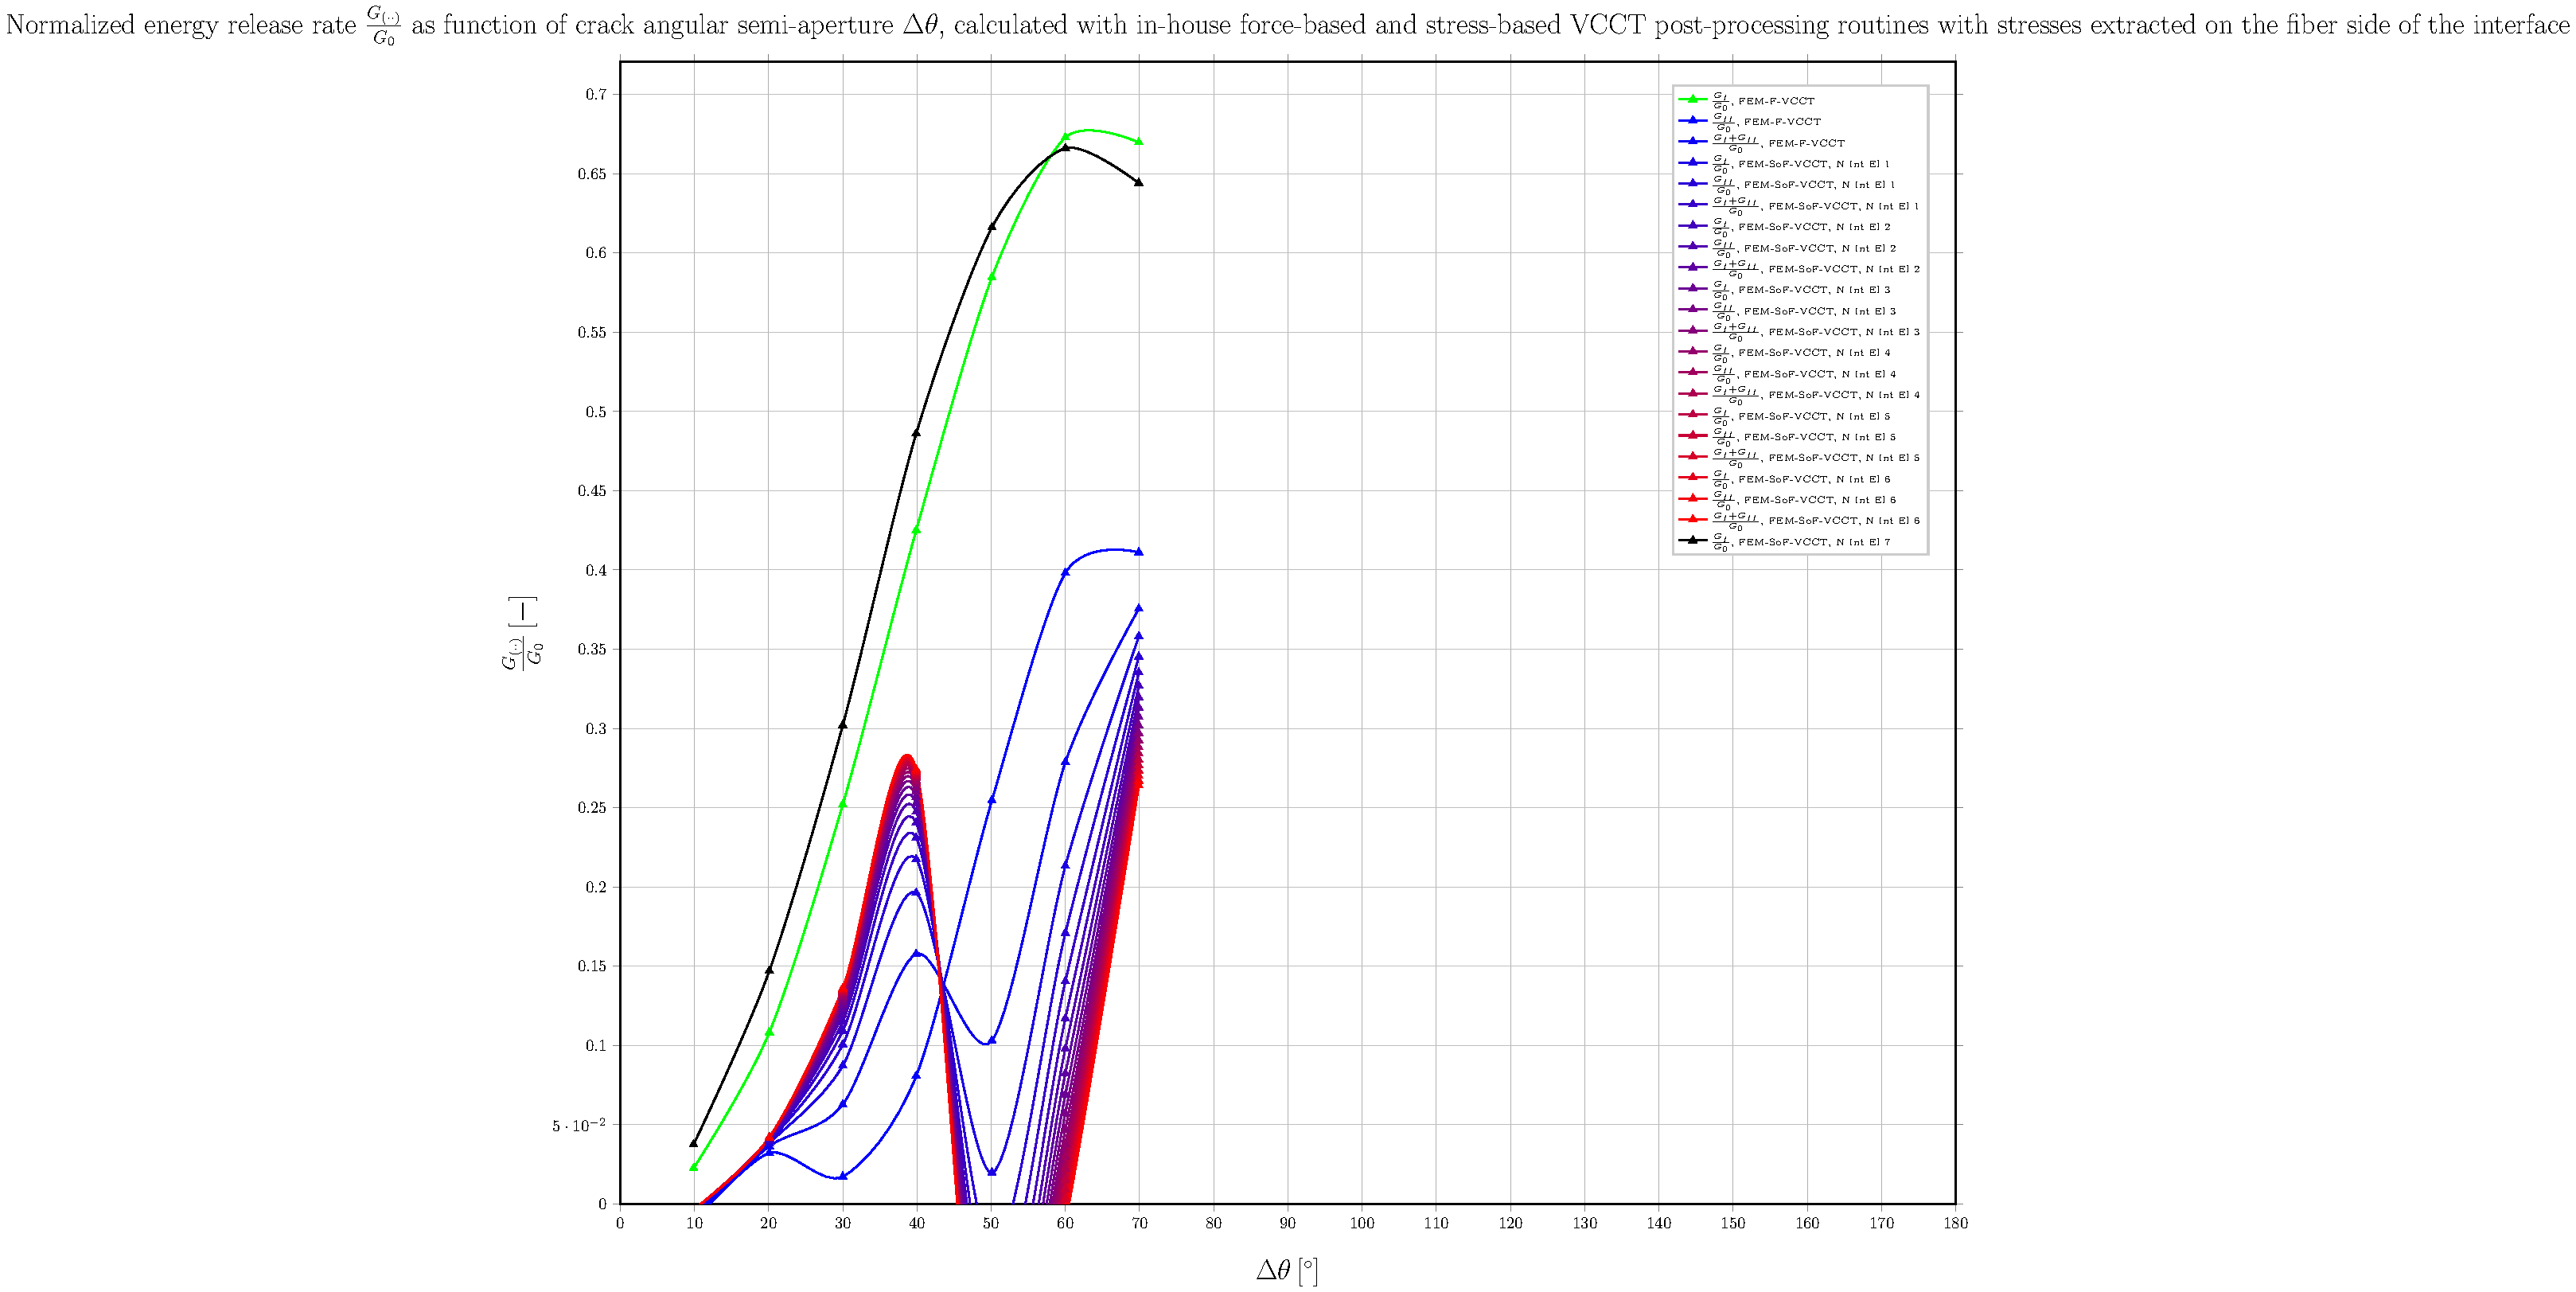
\includegraphics[height=0.7\textheight]{2017-07-25_AbqRunSummary_SmallStrain_D03/pdf/2017-07-25_AbqRunSummary_SmallStrain_D03_F-SoF-VCCT_GII.pdf}
  \caption{\scriptsize Fading from blue to red for increasing number of integration elements, Virtual Crack Closure Integral (VCCI) from FEM results; in green VCCT from FEM results; in black BEM results.}
  \label{fig:res1}
\end{figure}
\end{frame}
%%%%%%%%%%%%%%%%%%%%%%%%%%%%%%%%%%%%%
\begin{frame}
\frametitle{\small $G_{TOT}$ from VCCI, stresses extracted on fiber surface, $\delta=3.0^{\circ}$}
\vspace{-0.75cm}
\centering
\captionsetup[figure]{font=scriptsize,labelfont=scriptsize}
\begin{figure}[!h]
\centering
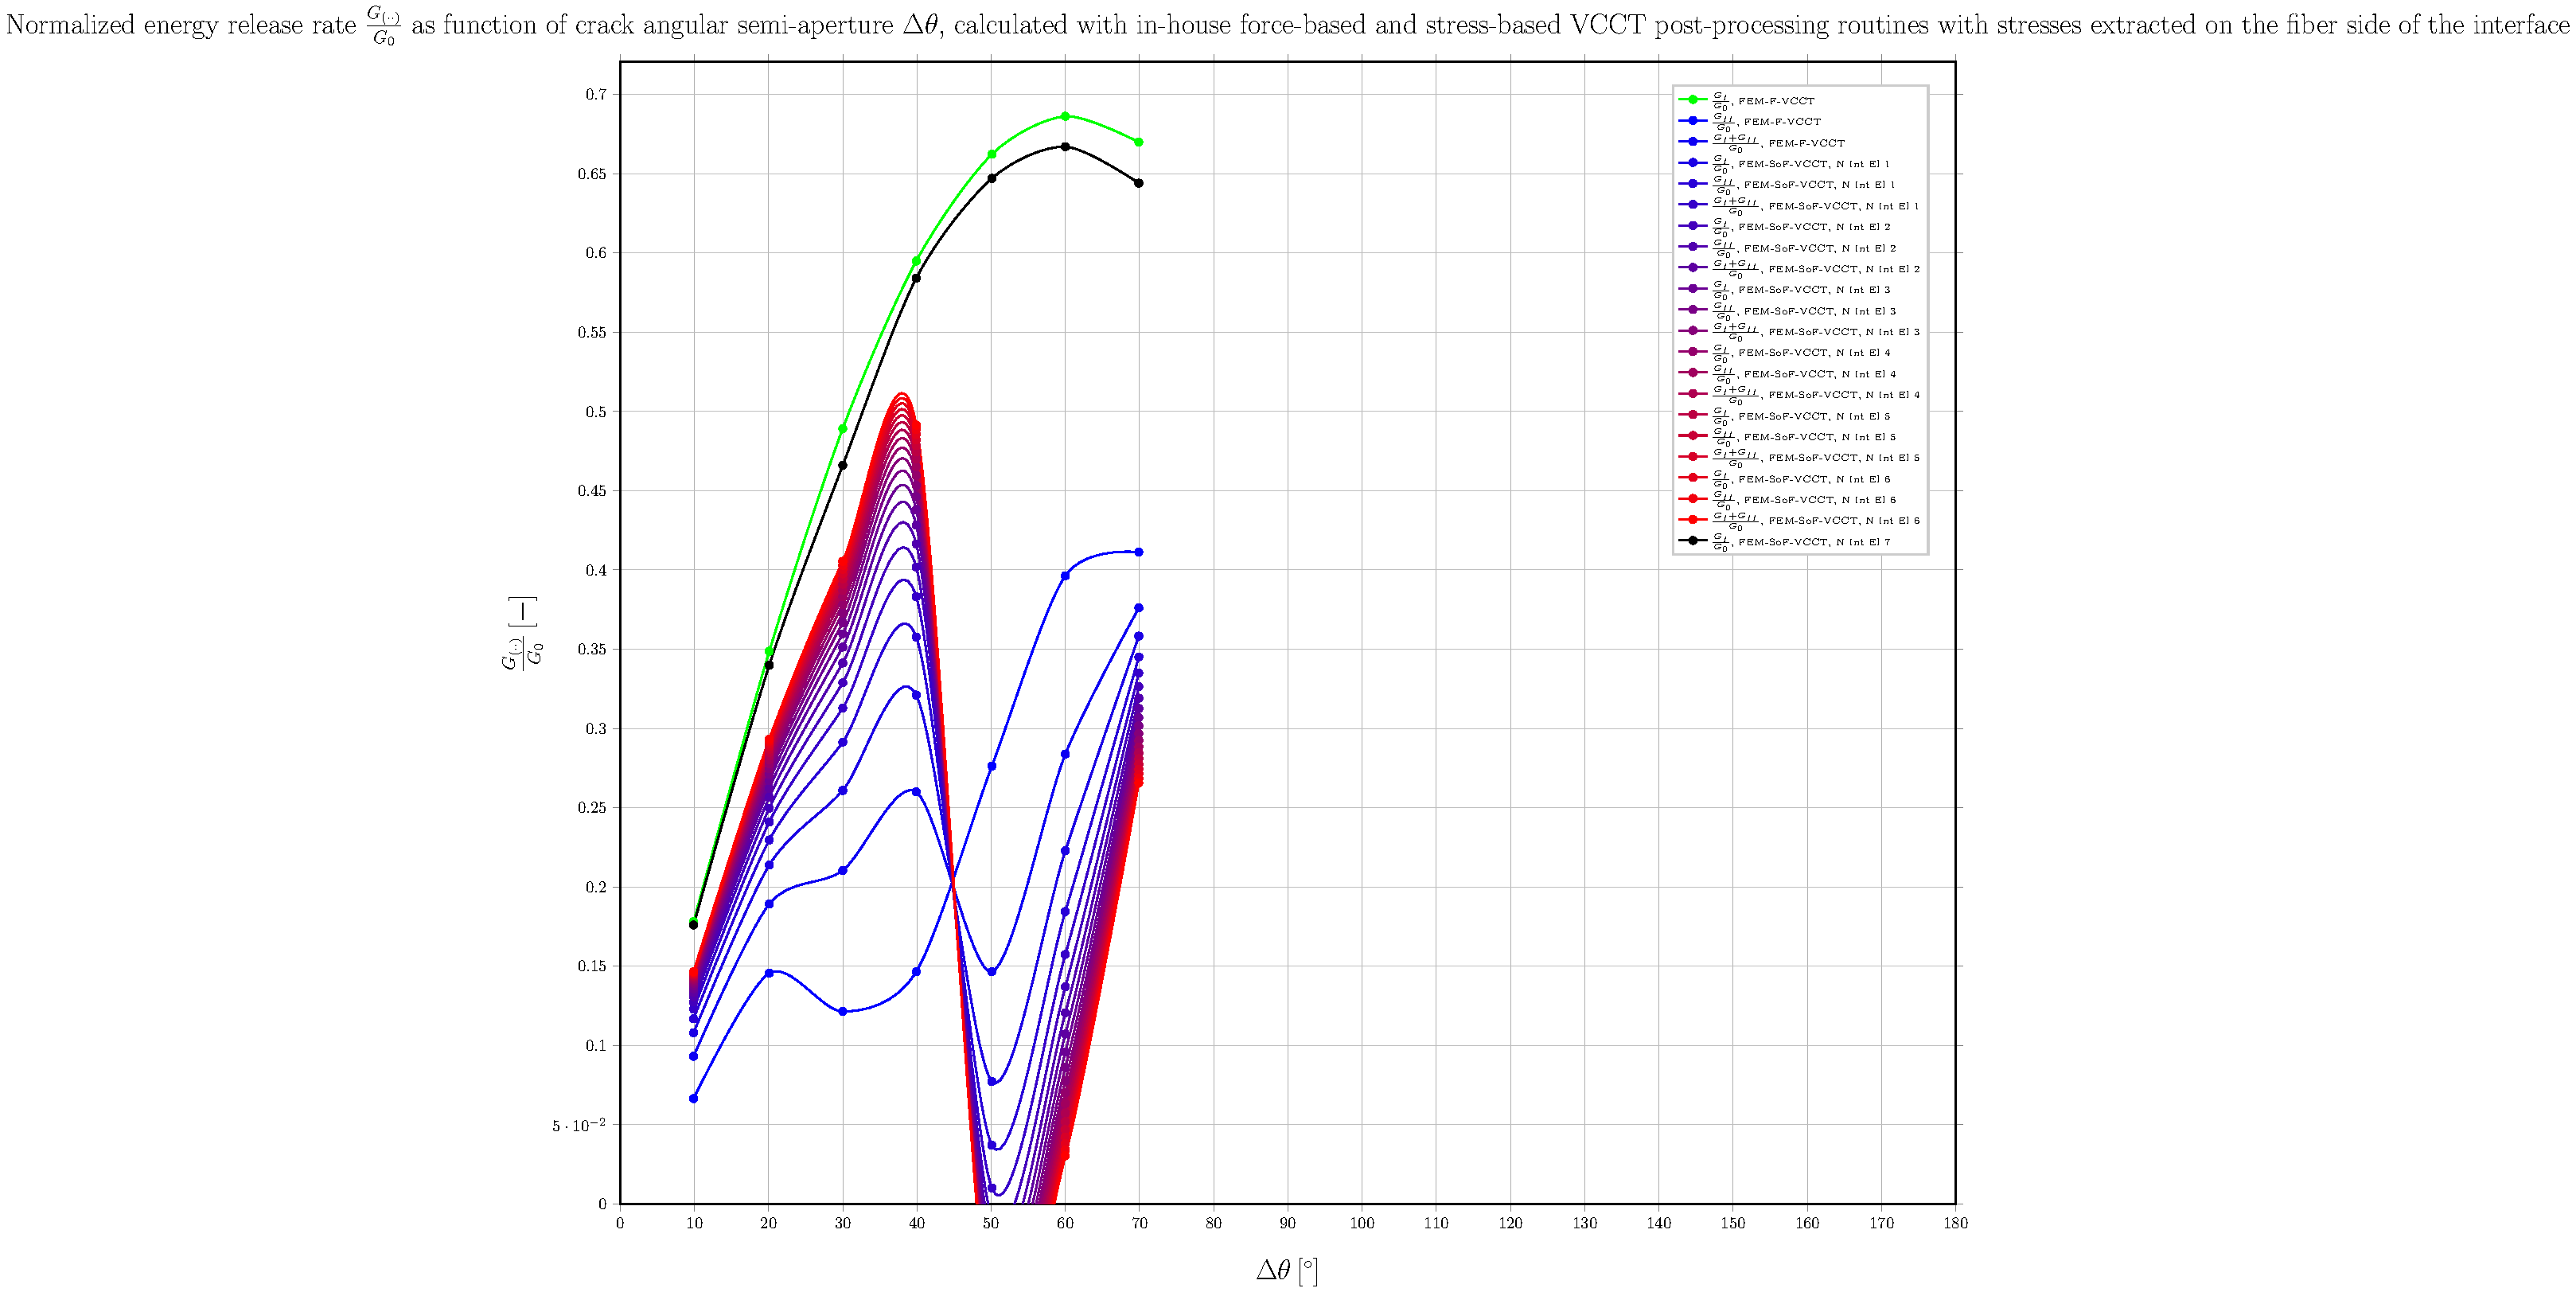
\includegraphics[height=0.7\textheight]{2017-07-25_AbqRunSummary_SmallStrain_D03/pdf/2017-07-25_AbqRunSummary_SmallStrain_D03_F-SoF-VCCT_GTOT.pdf}
  \caption{\scriptsize Fading from blue to red for increasing number of integration elements, Virtual Crack Closure Integral (VCCI) from FEM results; in green VCCT from FEM results; in black BEM results.}
  \label{fig:res1}
\end{figure}
\end{frame}
%%%%%%%%%%%%%%%%%%%%%%%%%%%%%%%%%%%%%
\begin{frame}
\frametitle{\small Summary of $G_{\left(\cdot\cdot\right)}$ from VCCI, stresses extracted on fiber surface, $\delta=3.0^{\circ}$}
\vspace{-0.75cm}
\centering
\captionsetup[figure]{font=scriptsize,labelfont=scriptsize}
\begin{figure}[!h]
\centering
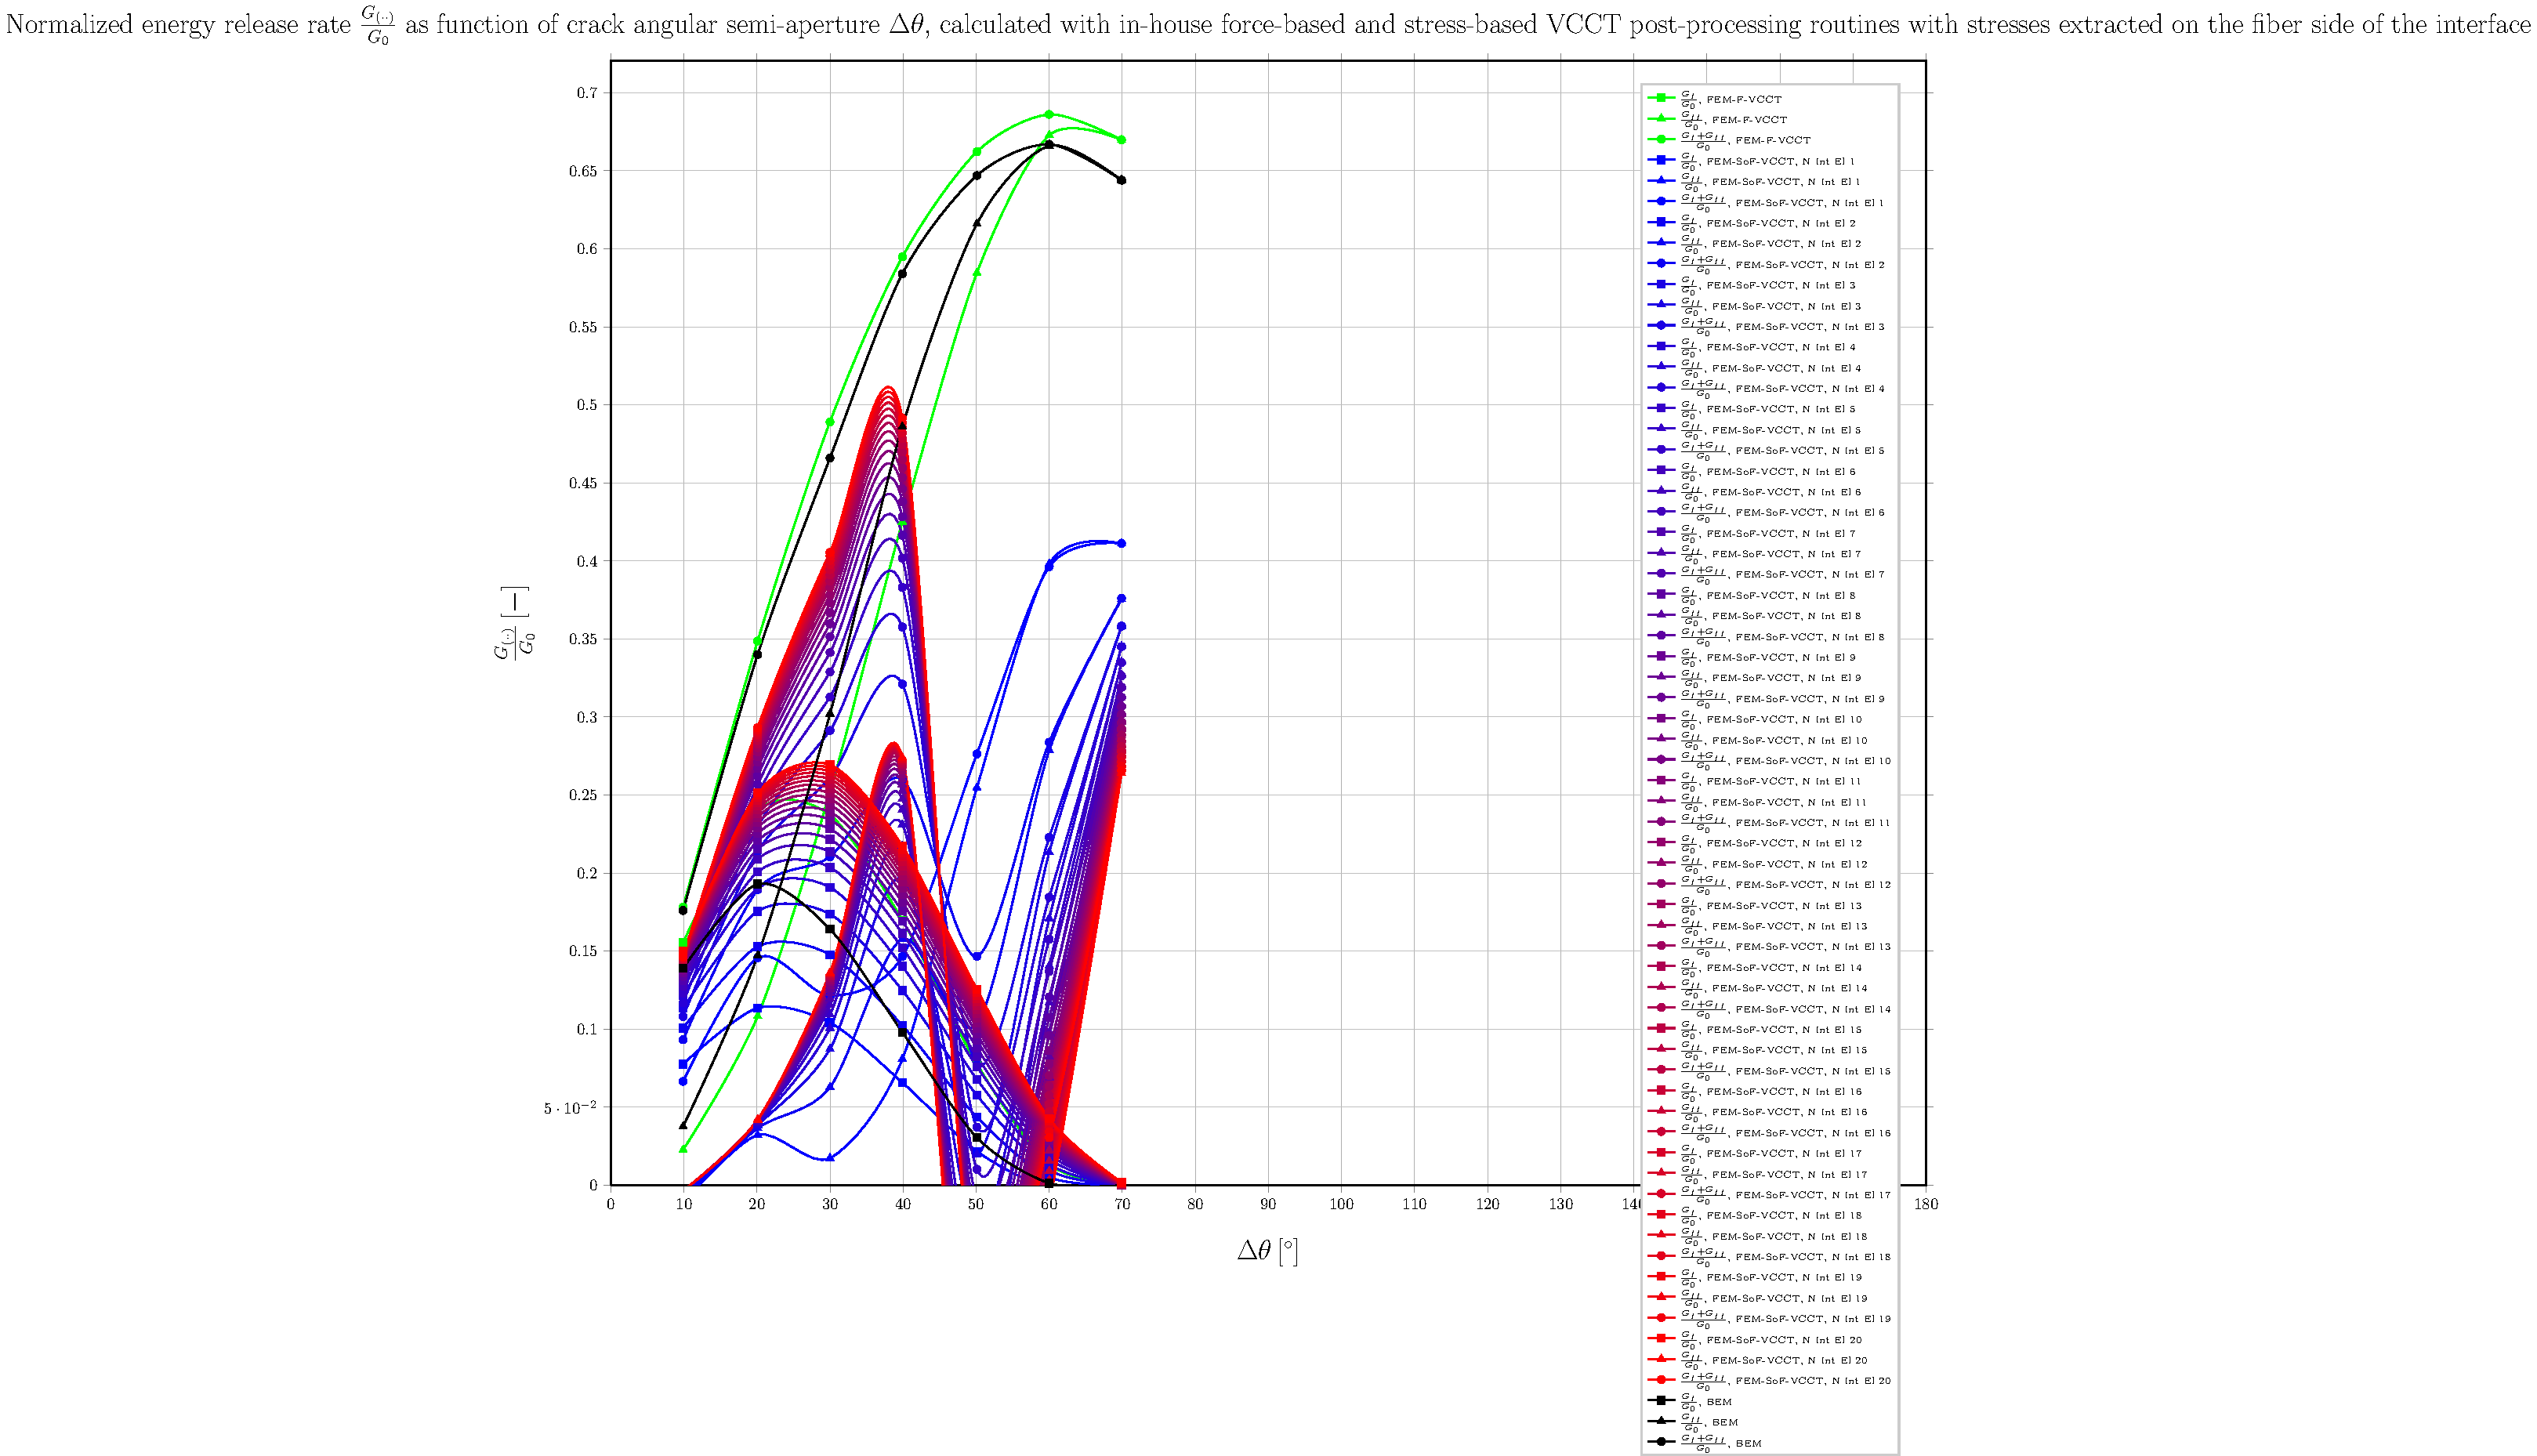
\includegraphics[height=0.7\textheight]{2017-07-25_AbqRunSummary_SmallStrain_D03/pdf/2017-07-25_AbqRunSummary_SmallStrain_D03_F-SoF-VCCT_Summary.pdf}
  \caption{\scriptsize Fading from blue to red for increasing number of integration elements, Virtual Crack Closure Integral (VCCI) from FEM results; in green VCCT from FEM results; in black BEM results.}
  \label{fig:res1}
\end{figure}
\end{frame}
%%%%%%%%%%%%%%%%%%%%%%%%%%%%%%%%%%%%%
\begin{frame}
\frametitle{\small $G_{I}$ from VCCI, stresses extracted on matrix surface, $\delta=3.0^{\circ}$}
\vspace{-0.75cm}
\centering
\captionsetup[figure]{font=scriptsize,labelfont=scriptsize}
\begin{figure}[!h]
\centering
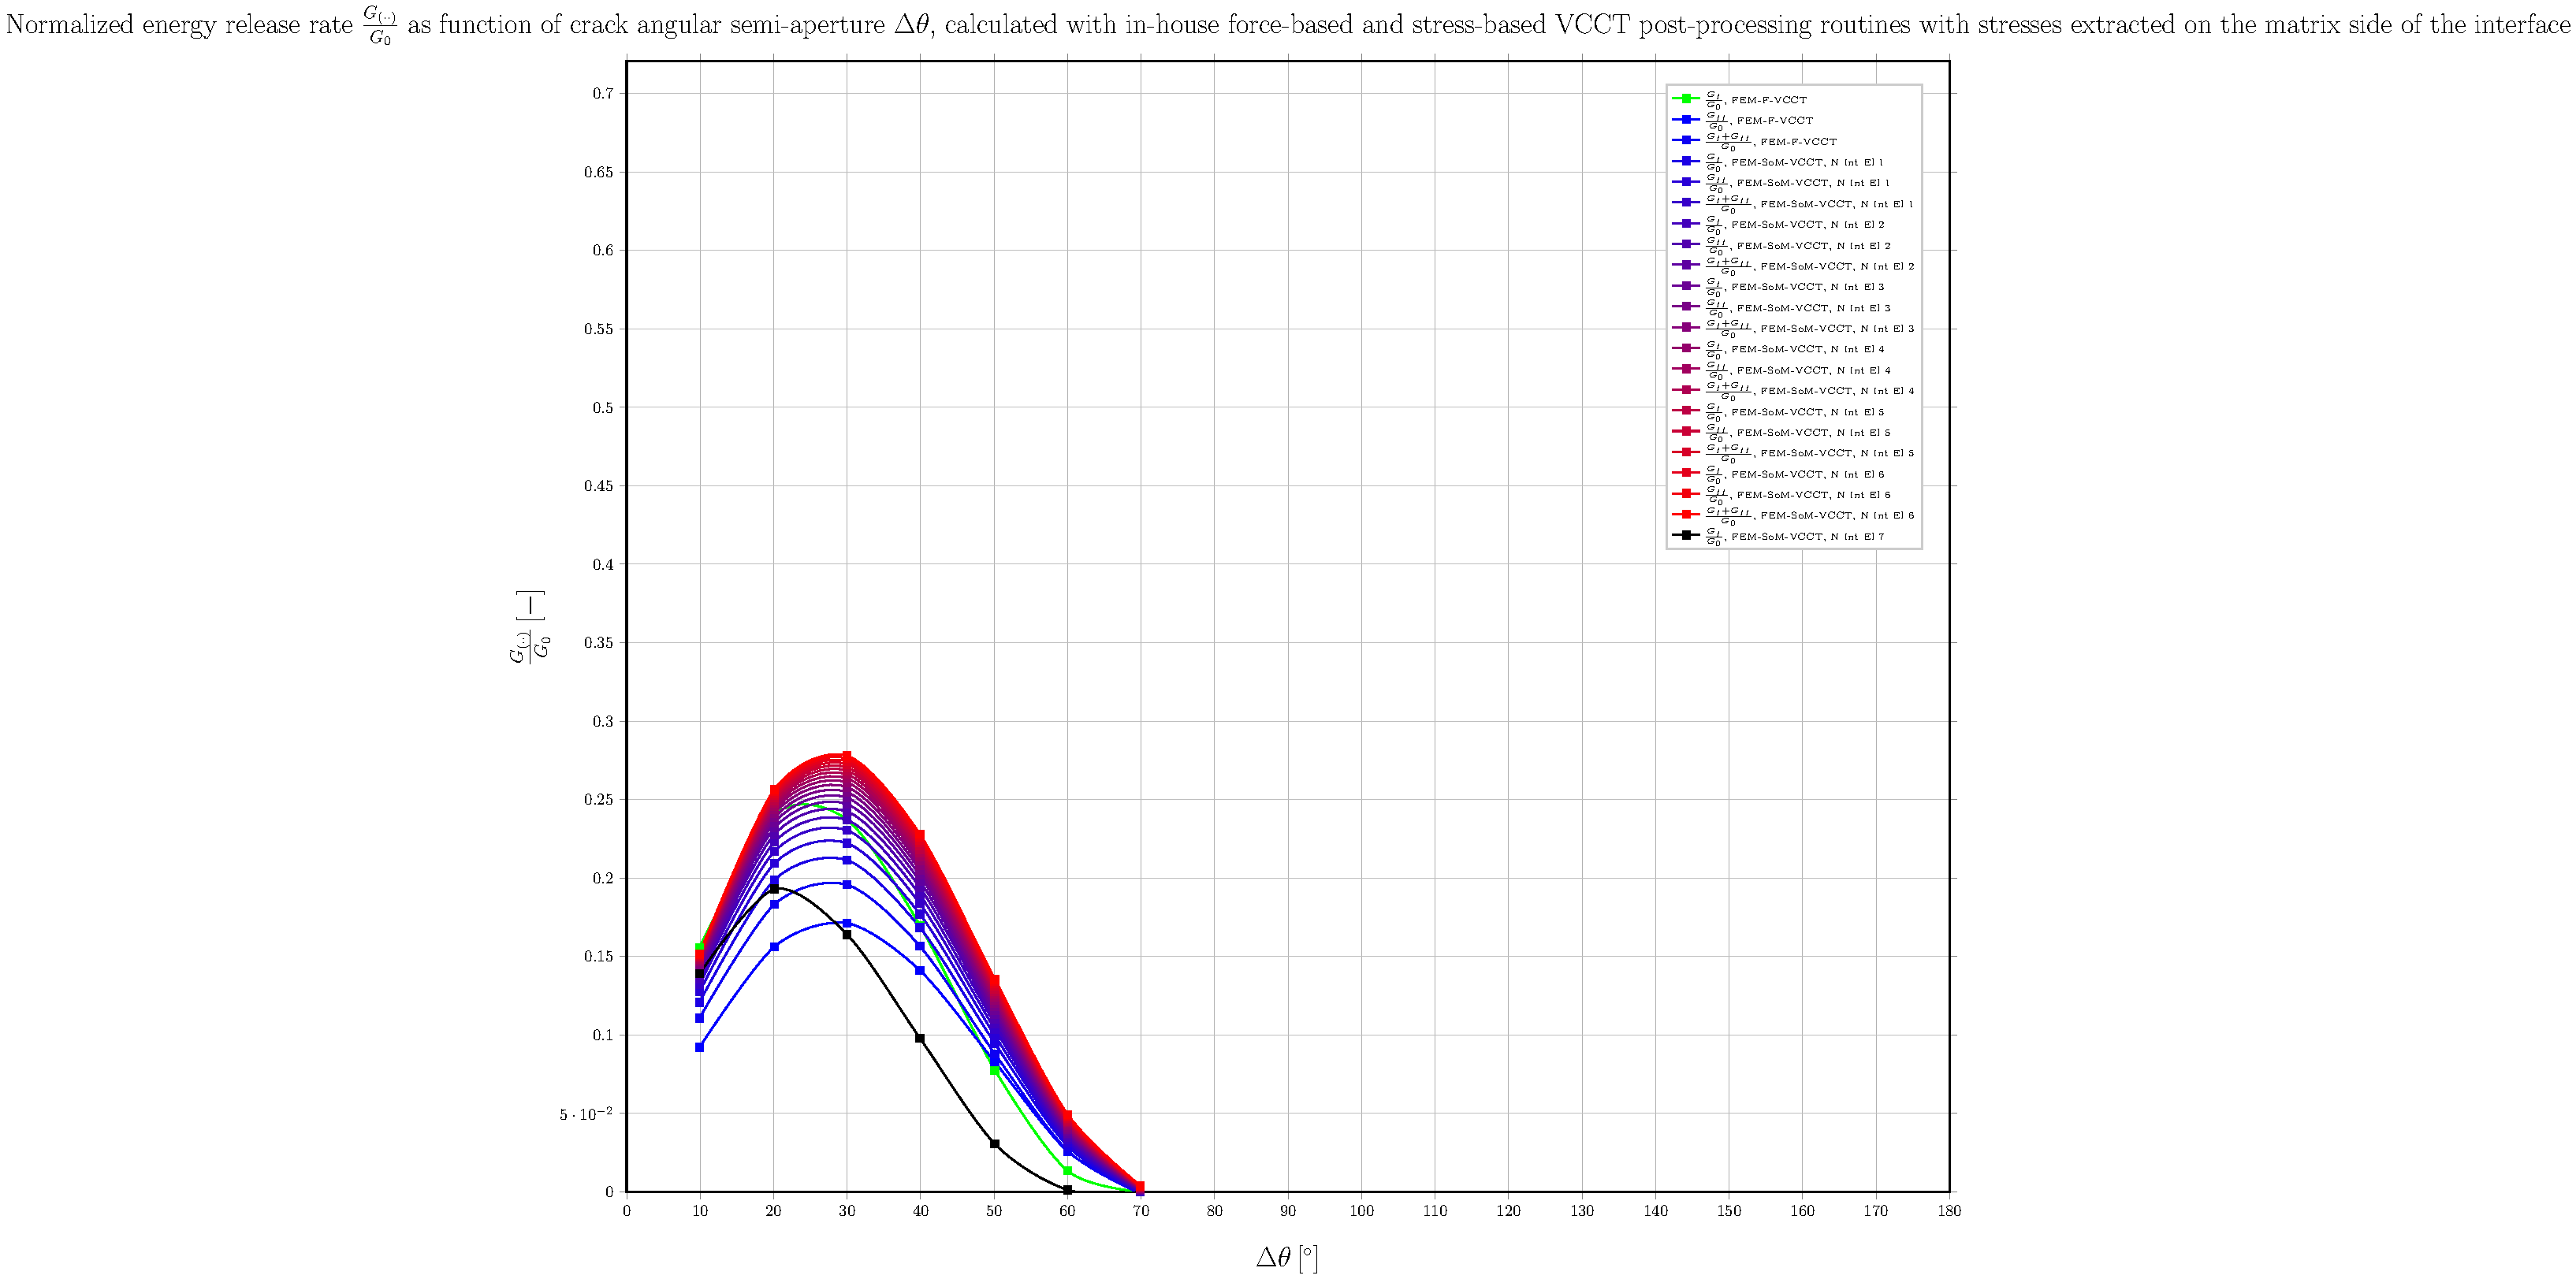
\includegraphics[height=0.7\textheight]{2017-07-25_AbqRunSummary_SmallStrain_D03/pdf/2017-07-25_AbqRunSummary_SmallStrain_D03_F-SoM-VCCT_GI.pdf}
  \caption{\scriptsize Fading from blue to red for increasing number of integration elements, Virtual Crack Closure Integral (VCCI) from FEM results; in green VCCT from FEM results; in black BEM results.}
  \label{fig:res1}
\end{figure}
\end{frame}
%%%%%%%%%%%%%%%%%%%%%%%%%%%%%%%%%%%%%
\begin{frame}
\frametitle{\small $G_{II}$ from VCCI, stresses extracted on matrix surface, $\delta=3.0^{\circ}$}
\vspace{-0.75cm}
\centering
\captionsetup[figure]{font=scriptsize,labelfont=scriptsize}
\begin{figure}[!h]
\centering
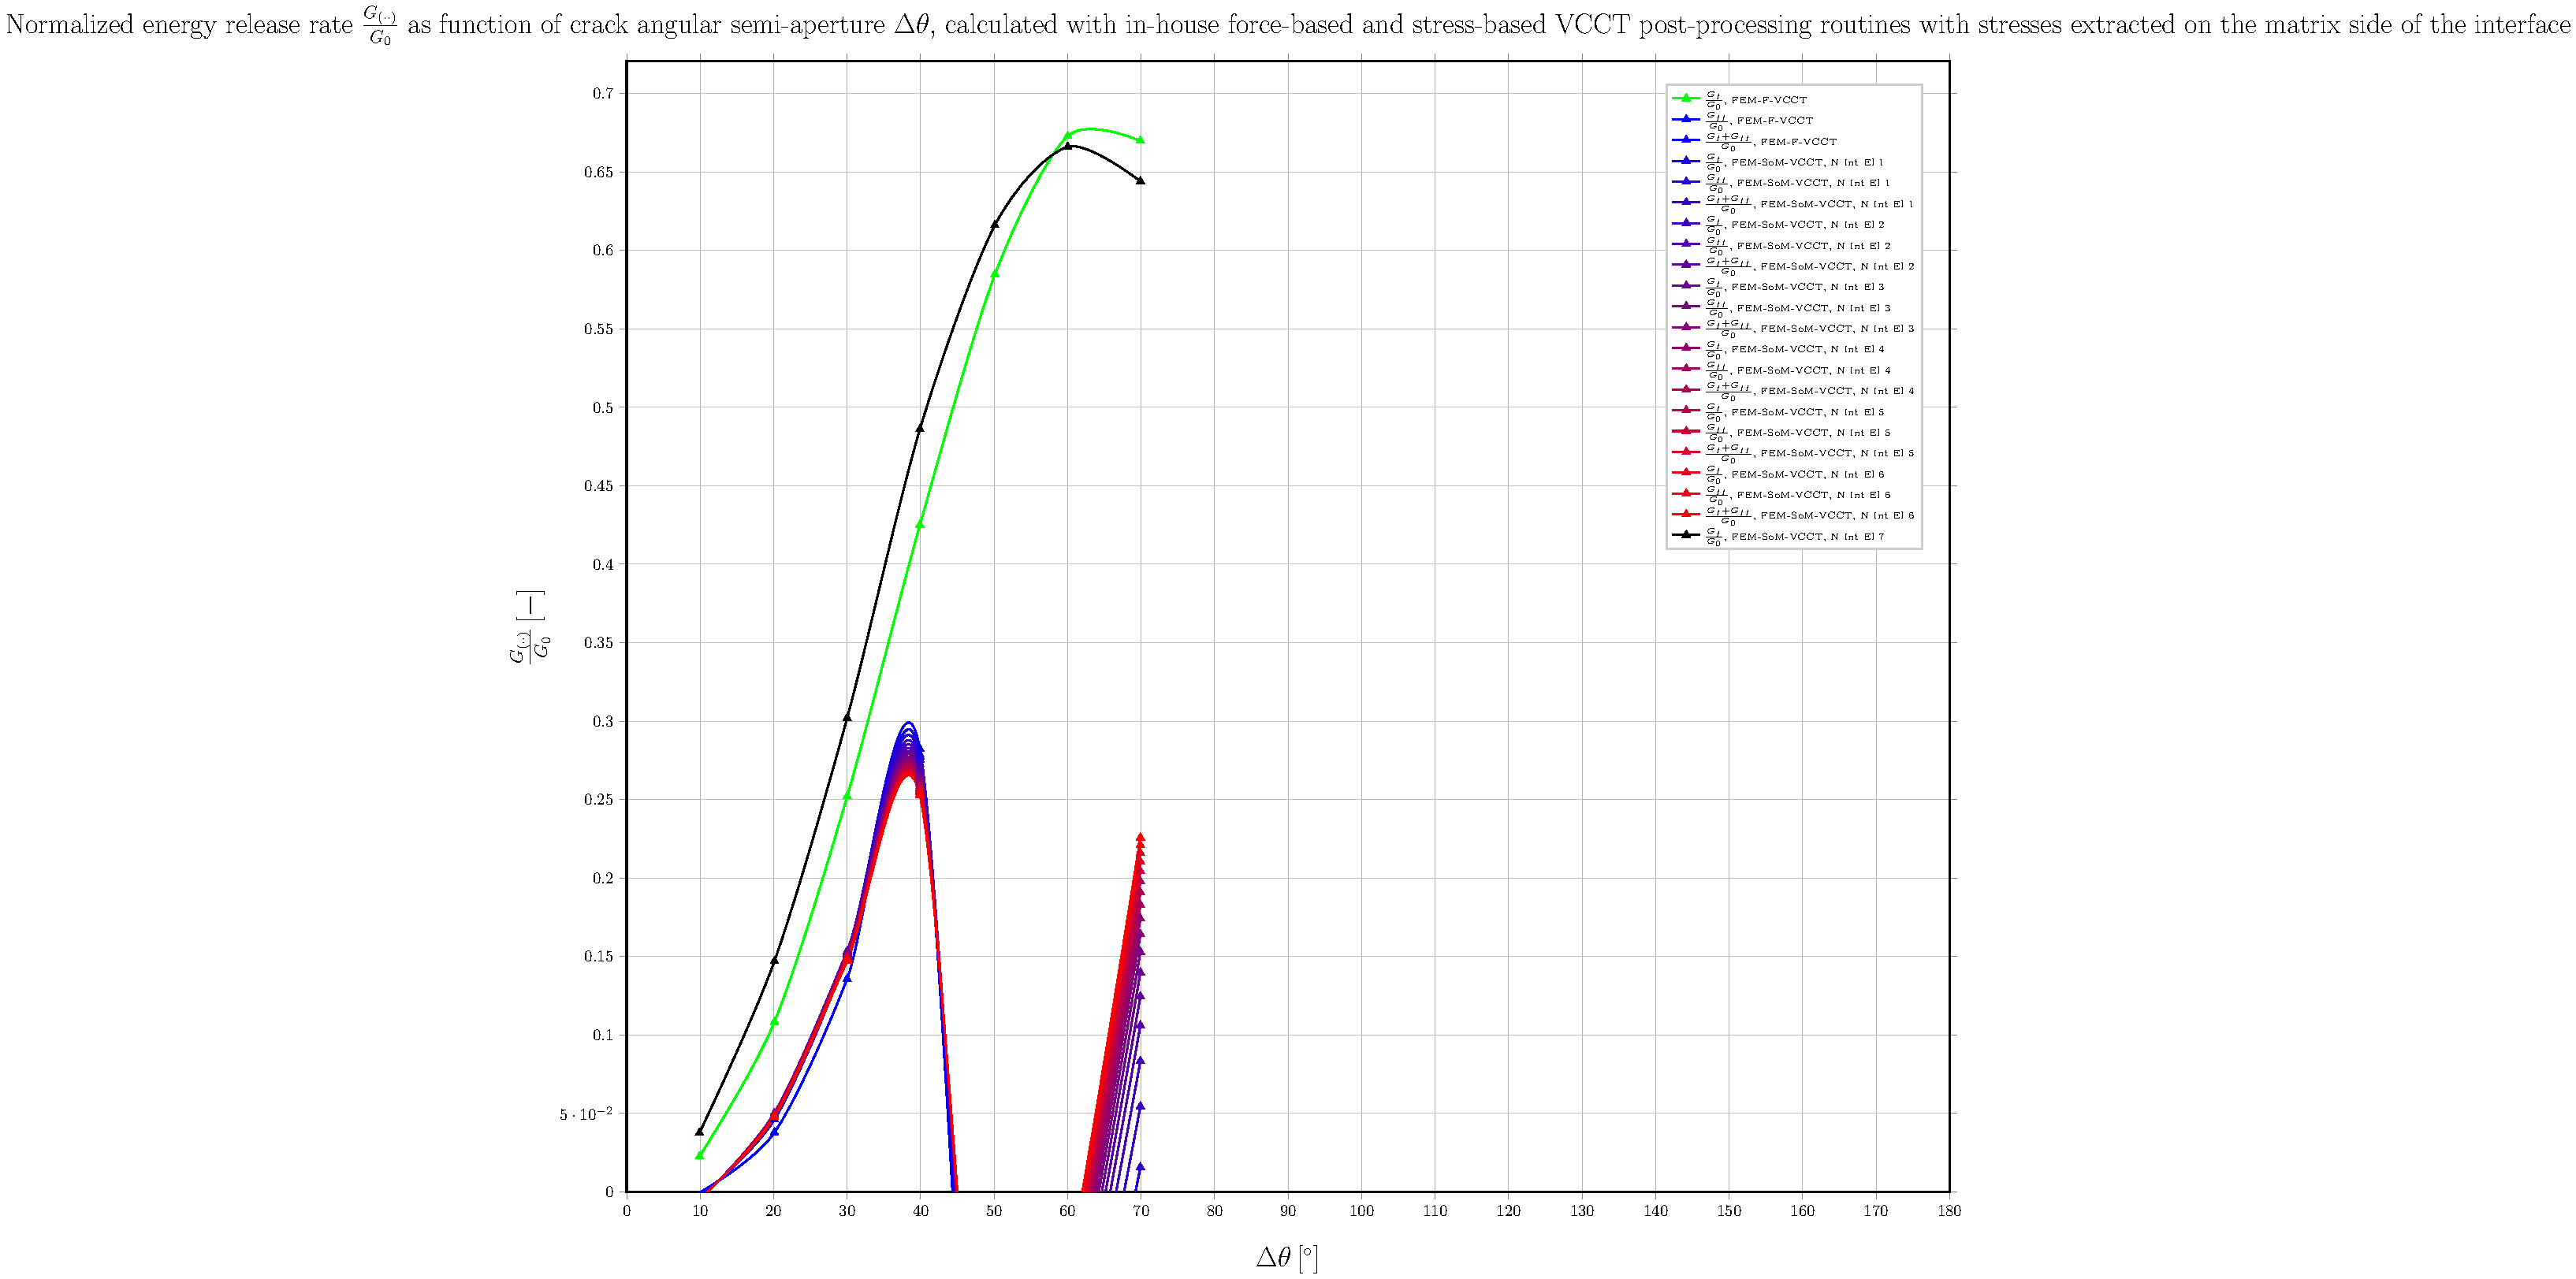
\includegraphics[height=0.7\textheight]{2017-07-25_AbqRunSummary_SmallStrain_D03/pdf/2017-07-25_AbqRunSummary_SmallStrain_D03_F-SoM-VCCT_GII.pdf}
  \caption{\scriptsize Fading from blue to red for increasing number of integration elements, Virtual Crack Closure Integral (VCCI) from FEM results; in green VCCT from FEM results; in black BEM results.}
  \label{fig:res1}
\end{figure}
\end{frame}
%%%%%%%%%%%%%%%%%%%%%%%%%%%%%%%%%%%%%
\begin{frame}
\frametitle{\small $G_{TOT}$ from VCCI, stresses extracted on matrix surface, $\delta=3.0^{\circ}$}
\vspace{-0.75cm}
\centering
\captionsetup[figure]{font=scriptsize,labelfont=scriptsize}
\begin{figure}[!h]
\centering
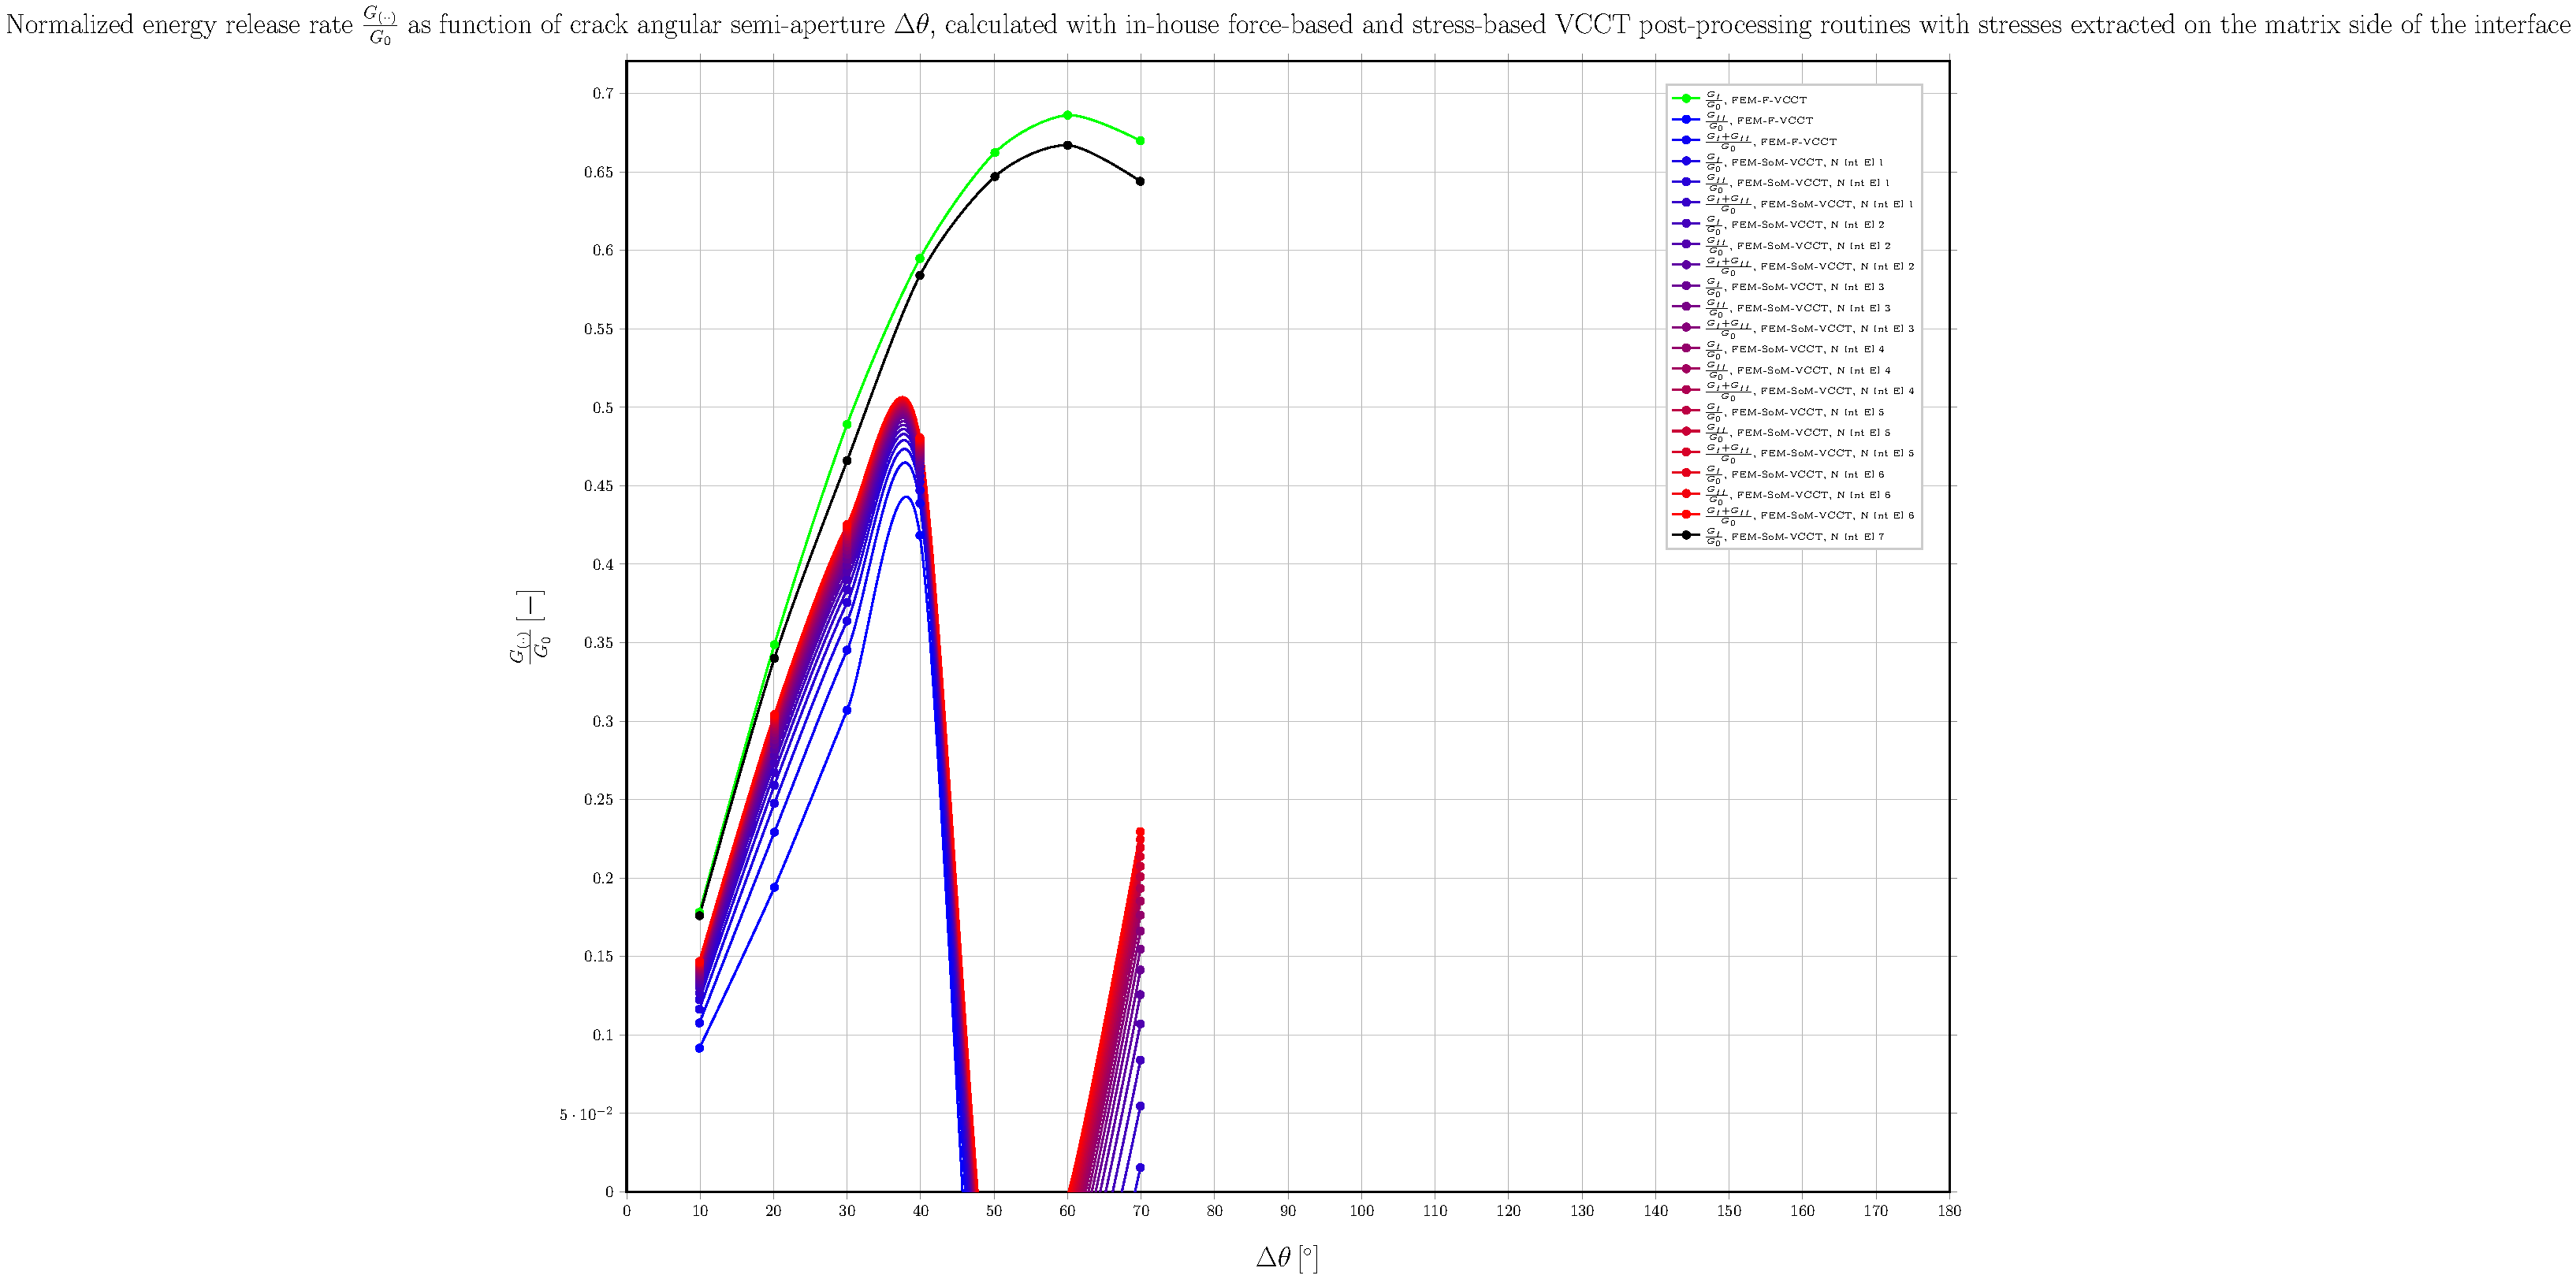
\includegraphics[height=0.7\textheight]{2017-07-25_AbqRunSummary_SmallStrain_D03/pdf/2017-07-25_AbqRunSummary_SmallStrain_D03_F-SoM-VCCT_GTOT.pdf}
  \caption{\scriptsize Fading from blue to red for increasing number of integration elements, Virtual Crack Closure Integral (VCCI) from FEM results; in green VCCT from FEM results; in black BEM results.}
  \label{fig:res1}
\end{figure}
\end{frame}
%%%%%%%%%%%%%%%%%%%%%%%%%%%%%%%%%%%%%
\begin{frame}
\frametitle{\small Summary of $G_{\left(\cdot\cdot\right)}$ from VCCI, stresses extracted on matrix surface, $\delta=3.0^{\circ}$}
\vspace{-0.75cm}
\centering
\captionsetup[figure]{font=scriptsize,labelfont=scriptsize}
\begin{figure}[!h]
\centering
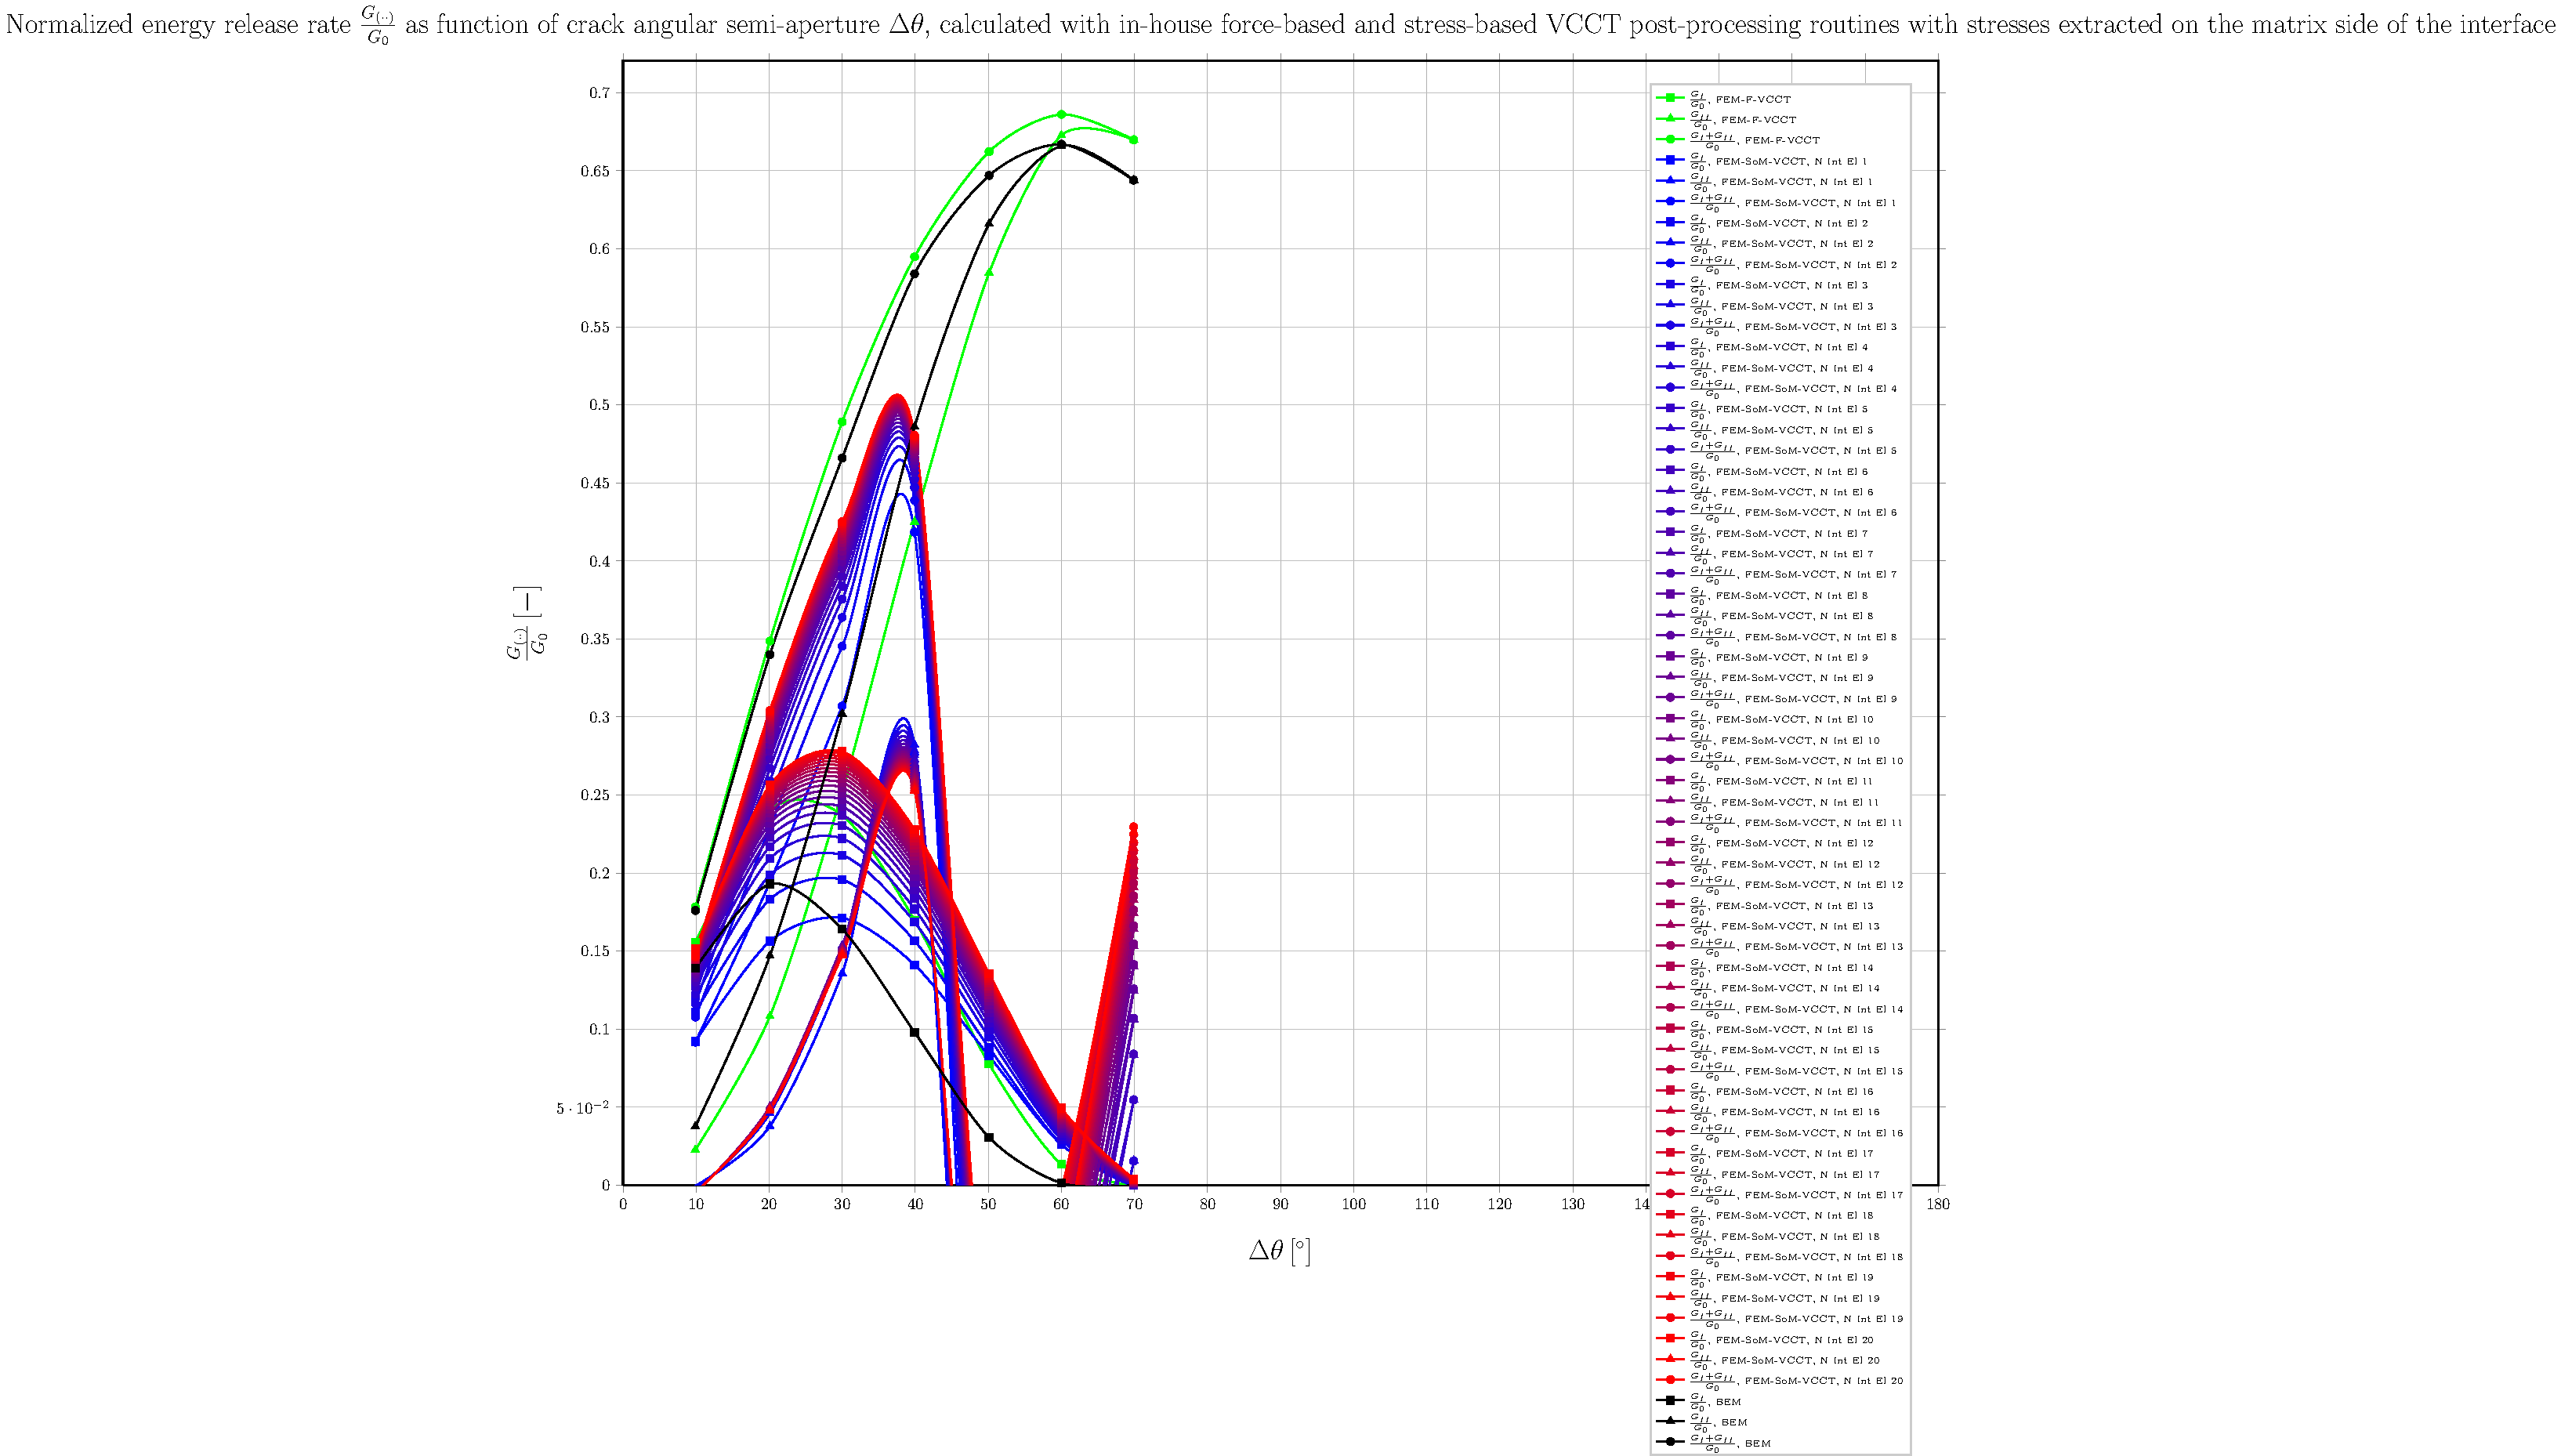
\includegraphics[height=0.7\textheight]{2017-07-25_AbqRunSummary_SmallStrain_D03/pdf/2017-07-25_AbqRunSummary_SmallStrain_D03_F-SoM-VCCT_Summary.pdf}
  \caption{\scriptsize Fading from blue to red for increasing number of integration elements, Virtual Crack Closure Integral (VCCI) from FEM results; in green VCCT from FEM results; in black BEM results.}
  \label{fig:res1}
\end{figure}
\end{frame}
%%%%%%%%%%%%%%%%%%%%%%%%%%%%%%%%%%%%%
